% id: 139-19
% book: 100발100중 3-2 중간 · 01 3-2 중간(삼각비·삼각비의 활용·원과 직선·원주각·부록)
% section: 파이널 모의고사 2회
% figure: crop:fig-139-19.png
% answer: ③
% answer_source: 답지(빠른정답)
% variant_level: 0 (원본 전사)
% 이 파일은 build.mjs 가 items.json 에서 만든다. 고칠 때는 items.json 을 고친다.
\smash{\raisebox{1.5mm}{\dmkichul{100발100중 3-2 중간 139쪽 19번}}}
\noindent\begin{minipage}[t]{0.58\linewidth}\vspace{0pt}\raggedright 그림에서 $\seg{AB}$는 원~$\pt{O}$의 지름이고 $\angle\pt{APR}=55^\circ$일 때, $\angle\pt{BQR}$의 크기는? \mbox{[3점]}\end{minipage}\hfill\begin{minipage}[t]{0.4\linewidth}\vspace{0pt}\centering 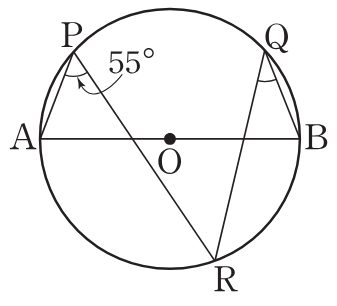
\includegraphics[width=80.6pt]{figures/fig-139-19.png}\end{minipage}\par
\begin{choicesii}{$25^\circ$}{$30^\circ$}{$35^\circ$}{$40^\circ$}{$45^\circ$}\end{choicesii}
